% Dueling DQN MLP architecture (used in v0, v1, rainbow_lite)
% Compile with: pdflatex arch_dueling.tex
\documentclass[tikz,border=2pt]{standalone}
\usepackage{amsmath}
\usetikzlibrary{arrows.meta,positioning,shapes.geometric,fit,backgrounds,calc}

\begin{document}
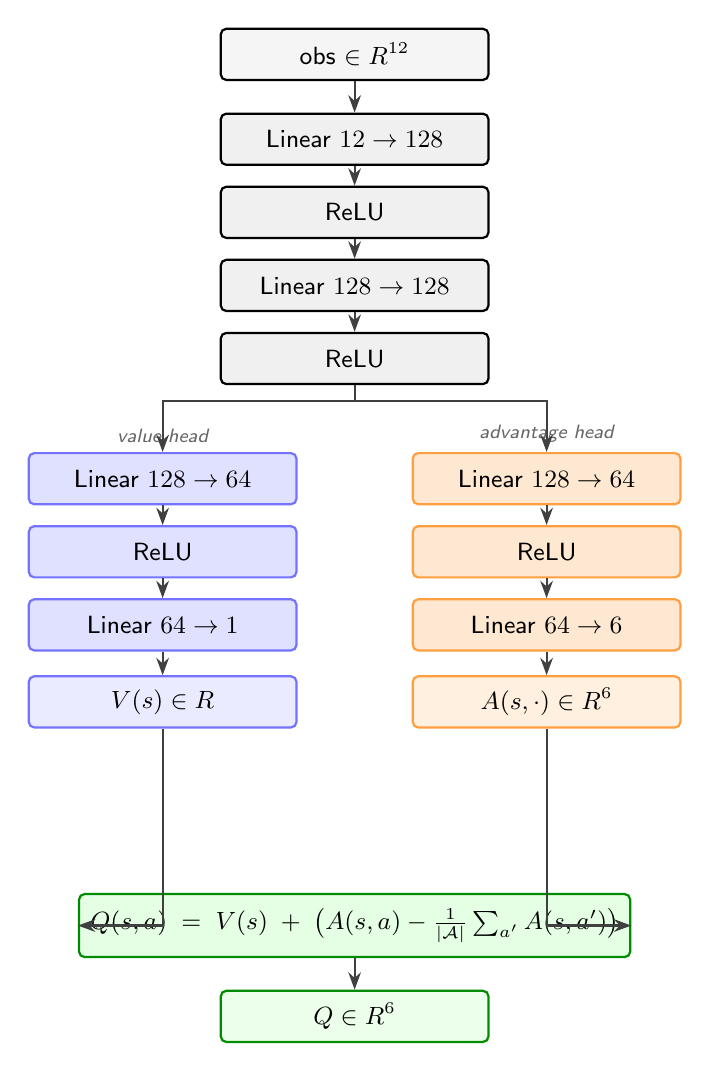
\begin{tikzpicture}[
  font=\sffamily\small,
  >={Stealth[length=2.2mm,width=1.6mm]},
  layer/.style={
    draw, rounded corners=2pt, thick,
    minimum width=34mm, minimum height=6.5mm,
    align=center, fill=gray!10
  },
  trunk/.style={layer, fill=gray!12},
  vlayer/.style={layer, fill=blue!12, draw=blue!55},
  alayer/.style={layer, fill=orange!18, draw=orange!75},
  io/.style={
    draw, thick, rounded corners=2pt,
    minimum width=34mm, minimum height=6.5mm,
    align=center, fill=black!4
  },
  combine/.style={
    draw, rounded corners=2pt, thick,
    minimum width=70mm, minimum height=8mm,
    align=center, fill=green!10, draw=green!55!black
  },
  arr/.style={->, thick, draw=black!75},
  branchlbl/.style={font=\sffamily\scriptsize\itshape, text=black!60}
]

% ---- input ----
\node[io] (in) {obs $\in \mathbb{R}^{12}$};

% ---- shared trunk ----
\node[trunk, below=4mm of in]    (fc1)   {Linear $12 \to 128$};
\node[trunk, below=2.5mm of fc1] (relu1) {ReLU};
\node[trunk, below=2.5mm of relu1] (fc2) {Linear $128 \to 128$};
\node[trunk, below=2.5mm of fc2] (relu2) {ReLU};

% ---- split point (invisible anchor) ----
\node[below=4mm of relu2] (split) {};

% ---- value head (left, blue) ----
\node[vlayer, below left=2mm and 6mm of split] (vfc1)  {Linear $128 \to 64$};
\node[vlayer, below=2.5mm of vfc1]             (vrelu) {ReLU};
\node[vlayer, below=2.5mm of vrelu]            (vfc2)  {Linear $64 \to 1$};
\node[io,    below=3mm of vfc2,
       fill=blue!8, draw=blue!55]              (vout)  {$V(s) \in \mathbb{R}$};

% ---- advantage head (right, orange) ----
\node[alayer, below right=2mm and 6mm of split] (afc1)  {Linear $128 \to 64$};
\node[alayer, below=2.5mm of afc1]              (arelu) {ReLU};
\node[alayer, below=2.5mm of arelu]             (afc2)  {Linear $64 \to 6$};
\node[io,    below=3mm of afc2,
       fill=orange!12, draw=orange!75]          (aout)  {$A(s,\cdot) \in \mathbb{R}^{6}$};

% ---- branch labels ----
\node[branchlbl, above=0pt of vfc1] {value head};
\node[branchlbl, above=0pt of afc1] {advantage head};

% ---- combination ----
\node[combine, below=12mm of split,
      yshift=-46mm] (comb)
   {$Q(s,a) \;=\; V(s) \;+\; \bigl(A(s,a) - \tfrac{1}{|\mathcal{A}|}\sum_{a'} A(s,a')\bigr)$};

% ---- output ----
\node[io, below=4mm of comb, fill=green!8, draw=green!55!black] (out)
   {$Q \in \mathbb{R}^{6}$};

% ---- arrows: trunk ----
\draw[arr] (in)    -- (fc1);
\draw[arr] (fc1)   -- (relu1);
\draw[arr] (relu1) -- (fc2);
\draw[arr] (fc2)   -- (relu2);

% split into two branches
\draw[arr] (relu2.south) -- ++(0,-2mm) -| (vfc1.north);
\draw[arr] (relu2.south) -- ++(0,-2mm) -| (afc1.north);

% value head chain
\draw[arr] (vfc1)  -- (vrelu);
\draw[arr] (vrelu) -- (vfc2);
\draw[arr] (vfc2)  -- (vout);

% advantage head chain
\draw[arr] (afc1)  -- (arelu);
\draw[arr] (arelu) -- (afc2);
\draw[arr] (afc2)  -- (aout);

% feed both into combine block
\draw[arr] (vout.south) |- (comb.west);
\draw[arr] (aout.south) |- (comb.east);

% combine -> output
\draw[arr] (comb) -- (out);

\end{tikzpicture}
\end{document}
